\chapter{Decision trees}
In decision trees each internal node corresponds to a feature, the branches correspond to a value of said feature and the leaves perform a prediction. 

It is composed of non-terminal nodes that have 2+ children and implement a {\bf routing function} and of leaf nodes which implement a prediction function.\\
A decision tree takes an input $x \in \mathscr{X}$ and routes it through the nodes until finding the final leaf, in which the prediction will take place.
\\
\\
Each non-terminal node is structured like so: \\
Node($\phi, T_L, T_R$), with a routing function $phi$ and the left and right trees underneath.
\\
On the other hand leaf nodes are Leaf(h), with h being a prediction function.
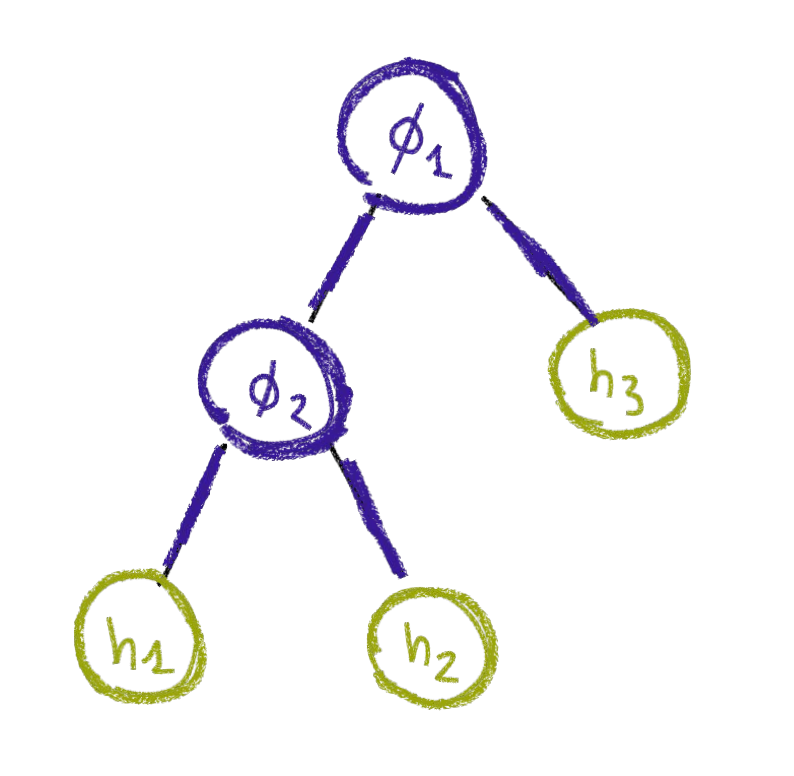
\includegraphics[scale=0.2]{dt}

\section{Growing the tree}
The main problem with growing the tree is whether we need to grow a node or a leaf. 

If a training set $\mathscr{D}$ is impure we will need to grow a node. On the other hand we will build a leaf if:

\[
I(\mathscr{D}) = E(h_{\mathscr{D}}^{\star}, \mathscr{D})
\]

As said previously if this stopping criterion is not met a node will be built with a routing function: 

\[
\phi_{\mathscr{D}}^\star \in argmin I_\phi (\mathscr{D})
\]

The impurity is computed in terms of the impurity of the split data.

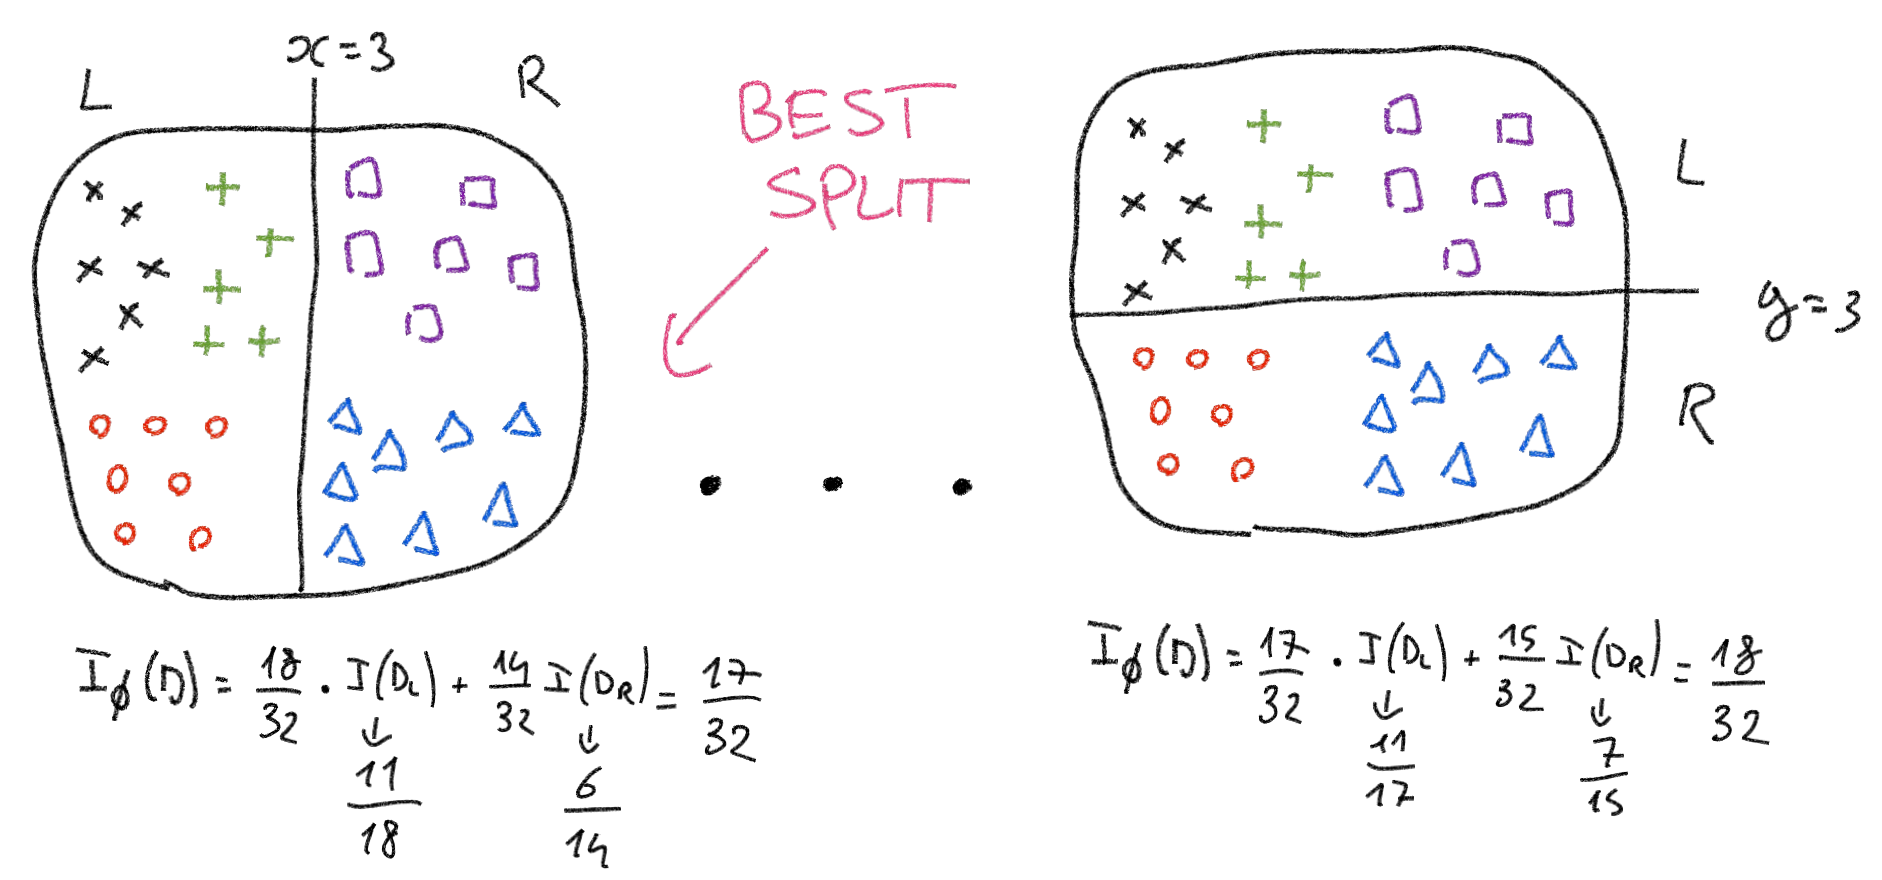
\includegraphics[scale=0.2]{split}

\section{Overfitting}
Because of the fact that they're determined by data, DT are particularly susceptible to overfitting. The usual techniques (regularization etc.) can be employed to avoid this, but there's also another called pruning.\\
This consists of taking a subtree and making it into a single node. This is usually done with subtress that are comprised of noisy data. \\
A {\bf random forest} is a collection of decision trees 